% Options for packages loaded elsewhere
\PassOptionsToPackage{unicode}{hyperref}
\PassOptionsToPackage{hyphens}{url}
\PassOptionsToPackage{dvipsnames,svgnames,x11names}{xcolor}
%
\documentclass[
]{agujournal2019}

\usepackage{amsmath,amssymb}
\usepackage{iftex}
\ifPDFTeX
  \usepackage[T1]{fontenc}
  \usepackage[utf8]{inputenc}
  \usepackage{textcomp} % provide euro and other symbols
\else % if luatex or xetex
  \usepackage{unicode-math}
  \defaultfontfeatures{Scale=MatchLowercase}
  \defaultfontfeatures[\rmfamily]{Ligatures=TeX,Scale=1}
\fi
\usepackage{lmodern}
\ifPDFTeX\else  
    % xetex/luatex font selection
\fi
% Use upquote if available, for straight quotes in verbatim environments
\IfFileExists{upquote.sty}{\usepackage{upquote}}{}
\IfFileExists{microtype.sty}{% use microtype if available
  \usepackage[]{microtype}
  \UseMicrotypeSet[protrusion]{basicmath} % disable protrusion for tt fonts
}{}
\makeatletter
\@ifundefined{KOMAClassName}{% if non-KOMA class
  \IfFileExists{parskip.sty}{%
    \usepackage{parskip}
  }{% else
    \setlength{\parindent}{0pt}
    \setlength{\parskip}{6pt plus 2pt minus 1pt}}
}{% if KOMA class
  \KOMAoptions{parskip=half}}
\makeatother
\usepackage{xcolor}
\setlength{\emergencystretch}{3em} % prevent overfull lines
\setcounter{secnumdepth}{5}
% Make \paragraph and \subparagraph free-standing
\makeatletter
\ifx\paragraph\undefined\else
  \let\oldparagraph\paragraph
  \renewcommand{\paragraph}{
    \@ifstar
      \xxxParagraphStar
      \xxxParagraphNoStar
  }
  \newcommand{\xxxParagraphStar}[1]{\oldparagraph*{#1}\mbox{}}
  \newcommand{\xxxParagraphNoStar}[1]{\oldparagraph{#1}\mbox{}}
\fi
\ifx\subparagraph\undefined\else
  \let\oldsubparagraph\subparagraph
  \renewcommand{\subparagraph}{
    \@ifstar
      \xxxSubParagraphStar
      \xxxSubParagraphNoStar
  }
  \newcommand{\xxxSubParagraphStar}[1]{\oldsubparagraph*{#1}\mbox{}}
  \newcommand{\xxxSubParagraphNoStar}[1]{\oldsubparagraph{#1}\mbox{}}
\fi
\makeatother


\providecommand{\tightlist}{%
  \setlength{\itemsep}{0pt}\setlength{\parskip}{0pt}}\usepackage{longtable,booktabs,array}
\usepackage{calc} % for calculating minipage widths
% Correct order of tables after \paragraph or \subparagraph
\usepackage{etoolbox}
\makeatletter
\patchcmd\longtable{\par}{\if@noskipsec\mbox{}\fi\par}{}{}
\makeatother
% Allow footnotes in longtable head/foot
\IfFileExists{footnotehyper.sty}{\usepackage{footnotehyper}}{\usepackage{footnote}}
\makesavenoteenv{longtable}
\usepackage{graphicx}
\makeatletter
\newsavebox\pandoc@box
\newcommand*\pandocbounded[1]{% scales image to fit in text height/width
  \sbox\pandoc@box{#1}%
  \Gscale@div\@tempa{\textheight}{\dimexpr\ht\pandoc@box+\dp\pandoc@box\relax}%
  \Gscale@div\@tempb{\linewidth}{\wd\pandoc@box}%
  \ifdim\@tempb\p@<\@tempa\p@\let\@tempa\@tempb\fi% select the smaller of both
  \ifdim\@tempa\p@<\p@\scalebox{\@tempa}{\usebox\pandoc@box}%
  \else\usebox{\pandoc@box}%
  \fi%
}
% Set default figure placement to htbp
\def\fps@figure{htbp}
\makeatother
% definitions for citeproc citations
\NewDocumentCommand\citeproctext{}{}
\NewDocumentCommand\citeproc{mm}{%
  \begingroup\def\citeproctext{#2}\cite{#1}\endgroup}
\makeatletter
 % allow citations to break across lines
 \let\@cite@ofmt\@firstofone
 % avoid brackets around text for \cite:
 \def\@biblabel#1{}
 \def\@cite#1#2{{#1\if@tempswa , #2\fi}}
\makeatother
\newlength{\cslhangindent}
\setlength{\cslhangindent}{1.5em}
\newlength{\csllabelwidth}
\setlength{\csllabelwidth}{3em}
\newenvironment{CSLReferences}[2] % #1 hanging-indent, #2 entry-spacing
 {\begin{list}{}{%
  \setlength{\itemindent}{0pt}
  \setlength{\leftmargin}{0pt}
  \setlength{\parsep}{0pt}
  % turn on hanging indent if param 1 is 1
  \ifodd #1
   \setlength{\leftmargin}{\cslhangindent}
   \setlength{\itemindent}{-1\cslhangindent}
  \fi
  % set entry spacing
  \setlength{\itemsep}{#2\baselineskip}}}
 {\end{list}}
\usepackage{calc}
\newcommand{\CSLBlock}[1]{\hfill\break\parbox[t]{\linewidth}{\strut\ignorespaces#1\strut}}
\newcommand{\CSLLeftMargin}[1]{\parbox[t]{\csllabelwidth}{\strut#1\strut}}
\newcommand{\CSLRightInline}[1]{\parbox[t]{\linewidth - \csllabelwidth}{\strut#1\strut}}
\newcommand{\CSLIndent}[1]{\hspace{\cslhangindent}#1}

\usepackage{url} %this package should fix any errors with URLs in refs.
\usepackage{lineno}
\usepackage[inline]{trackchanges} %for better track changes. finalnew option will compile document with changes incorporated.
\usepackage{soul}
\linenumbers
\makeatletter
\@ifpackageloaded{caption}{}{\usepackage{caption}}
\AtBeginDocument{%
\ifdefined\contentsname
  \renewcommand*\contentsname{Table of contents}
\else
  \newcommand\contentsname{Table of contents}
\fi
\ifdefined\listfigurename
  \renewcommand*\listfigurename{List of Figures}
\else
  \newcommand\listfigurename{List of Figures}
\fi
\ifdefined\listtablename
  \renewcommand*\listtablename{List of Tables}
\else
  \newcommand\listtablename{List of Tables}
\fi
\ifdefined\figurename
  \renewcommand*\figurename{Figure}
\else
  \newcommand\figurename{Figure}
\fi
\ifdefined\tablename
  \renewcommand*\tablename{Table}
\else
  \newcommand\tablename{Table}
\fi
}
\@ifpackageloaded{float}{}{\usepackage{float}}
\floatstyle{ruled}
\@ifundefined{c@chapter}{\newfloat{codelisting}{h}{lop}}{\newfloat{codelisting}{h}{lop}[chapter]}
\floatname{codelisting}{Listing}
\newcommand*\listoflistings{\listof{codelisting}{List of Listings}}
\makeatother
\makeatletter
\makeatother
\makeatletter
\@ifpackageloaded{caption}{}{\usepackage{caption}}
\@ifpackageloaded{subcaption}{}{\usepackage{subcaption}}
\makeatother

\usepackage{bookmark}

\IfFileExists{xurl.sty}{\usepackage{xurl}}{} % add URL line breaks if available
\urlstyle{same} % disable monospaced font for URLs
\hypersetup{
  pdftitle={Diferencias sexuales en especies de pingüinos de la Antártida: un análisis basado en características morfológicas},
  pdfauthor={Juana Perez Rodríguez; Simona Cruz García},
  pdfkeywords={Dimorfismo sexual, Pingüinos Pygoscelis},
  colorlinks=true,
  linkcolor={blue},
  filecolor={Maroon},
  citecolor={Blue},
  urlcolor={Blue},
  pdfcreator={LaTeX via pandoc}}


\journalname{Earth and Space Science}

\draftfalse

\begin{document}
\title{Diferencias sexuales en especies de pingüinos de la Antártida: un
análisis basado en características morfológicas}

\authors{Juana Perez Rodríguez\affil{1}, Simona Cruz García\affil{1}}
\affiliation{1}{ENES Unidad Morelia, }
\correspondingauthor{Juana Perez
Rodríguez}{jprodriguez@enesmorelia.unam.com}


\begin{abstract}
El dimorfismo sexual es una consecuencia evolutiva de la selección
sexual y natural, manifestándose en diferencias morfológicas entre
machos y hembras de una misma especie (Darwin, 1871). En este estudio,
se evaluó si las características morfológicas pueden predecir el sexo de
tres especies de pingüinos (\emph{Pygoscelis}) en el Archipiélago
Palmer, Antártida. Se analizaron datos de longitud y profundidad del
pico, longitud de la aleta y masa corporal mediante modelos de regresión
logística y bosque aleatorio (Hastie et al., 2009). La regresión
logística tuvo un mejor rendimiento, con una exactitud de 0.857 y un
área bajo la curva ROC de 0.938. La profundidad del pico fue el mejor
predictor del sexo, con un aumento de 1 mm asociado con una probabilidad
casi cuatro veces mayor de que el individuo sea macho (Williams \&
Croxall, 2005). Este estudio demuestra que las características del pico
son indicadores confiables del sexo en pingüinos \emph{Pygoscelis},
facilitando estudios ecológicos y de comportamiento en estas especies.
\end{abstract}





\subsection{Introducción}\label{introducciuxf3n}

El dimorfismo sexual, o las diferencias morfológicas entre machos y
hembras de una misma especie, es una consecuencia evolutiva de la
selección sexual y la selección natural (Darwin, 1871; Trivers, 1972).
Estas diferencias pueden manifestarse en tamaño, coloración,
comportamiento o características físicas específicas. Comprender las
causas y consecuencias del dimorfismo sexual es importante para entender
la ecología, el comportamiento reproductivo y la evolución de las
especies (Andersson, 1994).

Sin embargo, sigue siendo incierto si es posible inferir el sexo de
ciertas especies animales a partir de sus características morfológicas.
Este estudio explora esta cuestión mediante el análisis de datos
morfológicos de tres especies de pingüinos (\emph{Pygoscelis})
recolectados en tres islas del Archipiélago Palmer, Antártida (Ainley,
2002). Este análisis busca determinar si las medidas corporales, como la
longitud y profundidad del pico, la longitud de la aleta y la masa
corporal, pueden predecir el sexo de los pingüinos.

\subsection{Métodos}\label{muxe9todos}

\subsubsection{Recolección de
muestras}\label{recolecciuxf3n-de-muestras}

El trabajo de campo fue realizado en el Archipiélago Palmer, al oeste de
la Península Antártica, cerca de la Isla Anvers (64°46′S, 64°03′W),
durante los veranos australes de 2007/08, 2008/09 y 2009/10 (Wilson et
al., 2018). Las muestras fueron recolectadas en tres islas específicas
Figura~\ref{fig-mapa-distribucion}:

\begin{itemize}
\tightlist
\item
  \textbf{Biscoe Island} (64°48′S, 63°46′W)\\
\item
  \textbf{Torgersen Island} (64°46′S, 64°04′W)\\
\item
  \textbf{Dream Island} (64°43′S, 64°13′W)
\end{itemize}

\begin{figure}[H]

\centering{

\pandocbounded{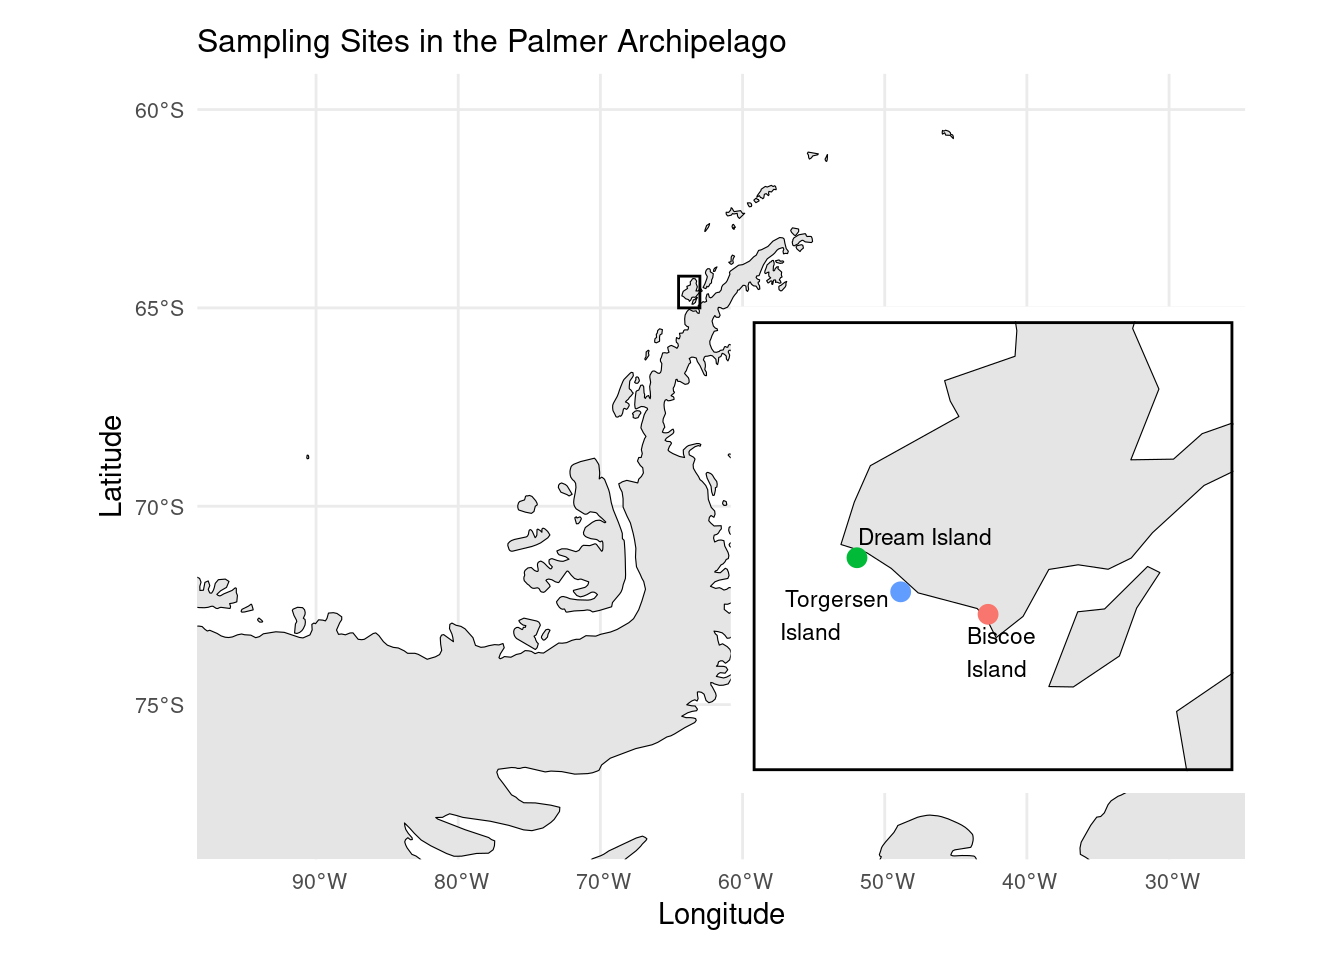
\includegraphics[keepaspectratio]{index_files/figure-latex/notebooks-DataExploration-fig-mapa-distribucion-output-2.png}}

}

\caption{\label{fig-mapa-distribucion}}

\end{figure}%

\textsubscript{Source:
\href{https://sofiazorrilla.github.io/Penguin_ms/notebooks/DataExploration-preview.html\#cell-fig-mapa-distribucion}{Exploración
de datos}}

Cada temporada, se recolectaron datos de 30 nidos de pingüinos Adelia,
distribuidos equitativamente entre las tres islas (10 nidos por isla).
Los datos de 30 nidos de pingüinos gentoo se recolectaron únicamente en
Biscoe Island, mientras que los datos de 15 nidos de pingüinos barbijo
fueron recolectados en Dream Island.

\begin{longtable}[]{@{}lllll@{}}

\caption{\label{tbl-sampling}Summary of Penguin Counts by Species,
Island, and Sex}

\tabularnewline

\toprule\noalign{}
Species & Island & Male & Female & Unkn. \\
\midrule\noalign{}
\endhead
\bottomrule\noalign{}
\endlastfoot
P. adelie & Torgersen & 23 & 24 & 5 \\
P. adelie & Biscoe & 22 & 22 & \\
P. adelie & Dream & 28 & 27 & 1 \\
P. gentoo & Biscoe & 61 & 58 & 5 \\
P. chinstrap & Dream & 34 & 34 & \\

\end{longtable}

\textsubscript{Source:
\href{https://sofiazorrilla.github.io/Penguin_ms/notebooks/DataExploration-preview.html\#cell-tbl-sampling}{Exploración
de datos}}

Las aves fueron capturadas en la etapa de un huevo, y se extrajo una
muestra de sangre (\textasciitilde1 ml) de la vena braquial utilizando
una jeringa estéril de 3 ml con aguja heparinizada (Lynch \& Schwaller,
2012). Las muestras de sangre fueron almacenadas en microtubos de 1.5 ml
y congeladas a -80°C para su análisis molecular y de isotopos estables.
Además, se registraron las siguientes medidas corporales:

\begin{itemize}
\tightlist
\item
  Longitud y profundidad del pico (mediante calibradores digitales ±0.1
  mm)\\
\item
  Longitud de la aleta (mediante regla ±1 mm)\\
\item
  Masa corporal (mediante balanzas de Pesola de 5 kg ±25 g o 10 kg ±50
  g)
\end{itemize}

\begin{figure}[H]

\centering{

\pandocbounded{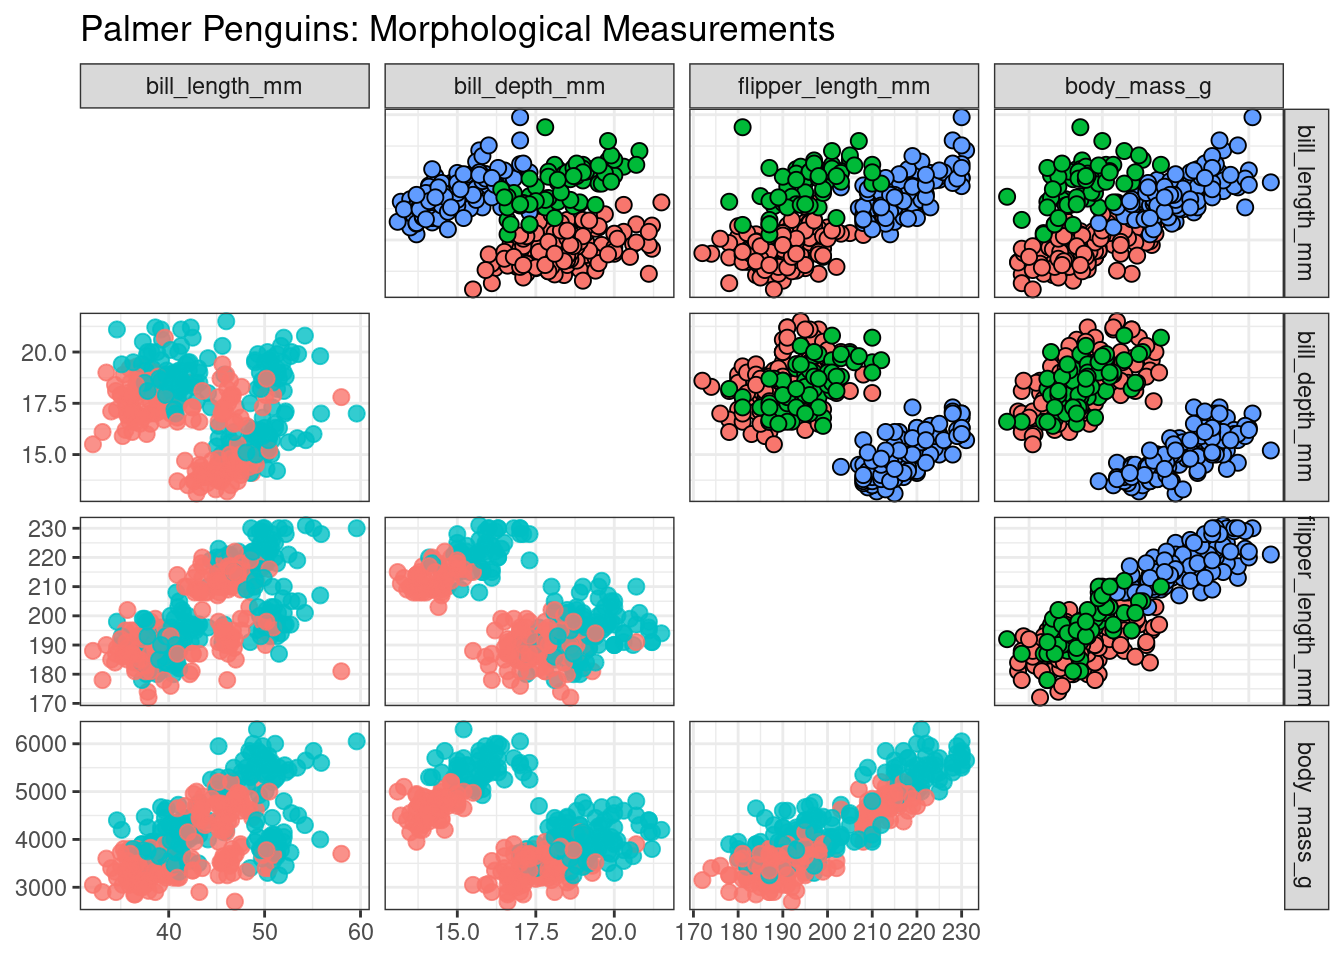
\includegraphics[keepaspectratio]{index_files/figure-latex/notebooks-DataExploration-fig-measureexploration-output-2.png}}

}

\caption{\label{fig-measureexploration}}

\end{figure}%

\textsubscript{Source:
\href{https://sofiazorrilla.github.io/Penguin_ms/notebooks/DataExploration-preview.html\#cell-fig-MeasureExploration}{Exploración
de datos}}

\subsubsection{Análisis estadístico}\label{anuxe1lisis-estaduxedstico}

Se construyeron modelos de regresión logística y de bosque aleatorio
para clasificar el sexo de los pingüinos basándose en las
características morfológicas (Hastie et al., 2009). La estructura de los
modelos fue la siguiente:

\begin{itemize}
\item
  \textbf{Regresión logística}:\\
  Modelo de clasificación utilizando la función \texttt{logistic\_reg()}
  en R, con el motor \texttt{glm}.
\item
  \textbf{Bosque aleatorio}:\\
  Modelo de clasificación utilizando \texttt{rand\_forest()} en R, con
  el motor \texttt{ranger}.
\end{itemize}

Se realizaron remuestreos mediante \texttt{bootstrapping} para evaluar
la estabilidad de los modelos y se midió la precisión mediante la
métrica de exactitud (\texttt{accuracy}) y el área bajo la curva ROC
(\texttt{roc\_auc}) (Breiman, 2001).

\subsection{Resultados}\label{resultados}

Los resultados muestran que el modelo de regresión logística tuvo un
mejor rendimiento que el modelo de bosque aleatorio. La exactitud y el
área bajo la curva ROC fueron las siguientes:

\begin{itemize}
\tightlist
\item
  \textbf{Exactitud}: 0.857\\
\item
  \textbf{ROC AUC}: 0.9382086
\end{itemize}

El análisis de razones de momios (\texttt{odds\ ratio}) indicó que la
mayor asociación con el sexo fue para la profundidad del pico, seguida
por la longitud del pico (Williams \& Croxall, 2005). Un aumento de 1 mm
en la profundidad del pico se asocia con una probabilidad casi cuatro
veces mayor de que el individuo sea macho. Por otro lado, la longitud de
la aleta no mostró evidencia significativa de diferenciación entre
machos y hembras cuando se controlaron las otras variables.

\subsection{Discusión}\label{discusiuxf3n}

La capacidad de inferir el sexo de los pingüinos a partir de datos
morfológicos tiene importantes implicaciones ecológicas y evolutivas
(Croxall, 1995). La diferenciación sexual basada en la morfología puede
estar relacionada con la selección sexual o con la adaptación a
diferentes roles ecológicos. La profundidad y longitud del pico pueden
reflejar diferencias en la dieta o en el comportamiento reproductivo
entre machos y hembras (Polito et al., 2016).

Además, la posibilidad de determinar el sexo mediante datos morfológicos
facilita estudios sobre dinámica poblacional y comportamiento
reproductivo, sin la necesidad de técnicas invasivas de determinación de
sexo (Polito et al., 2016).

\subsection{Conclusión}\label{conclusiuxf3n}

Este estudio demuestra que las características del pico son indicadores
confiables del sexo en especies de pingüinos \emph{Pygoscelis}. La
regresión logística proporcionó una alta exactitud y poder predictivo.
La capacidad de inferir el sexo a partir de datos morfológicos ofrece
nuevas oportunidades para estudios ecológicos y de comportamiento en
poblaciones de pingüinos en la Antártida (Trivelpiece et al., 2011).

\subsection*{Referencias}\label{referencias}
\addcontentsline{toc}{subsection}{Referencias}

\phantomsection\label{refs}
\begin{CSLReferences}{1}{0}
\vspace{1em}

\bibitem[\citeproctext]{ref-ainley2002}
Ainley, D. G. (2002). \emph{The ad{é}lie penguin: Bellwether of climate
change}. New York: Columbia University Press.

\bibitem[\citeproctext]{ref-andersson1994}
Andersson, M. (1994). \emph{Sexual selection}. Princeton: Princeton
University Press.

\bibitem[\citeproctext]{ref-breiman2001}
Breiman, L. (2001). Random forests. \emph{Machine Learning},
\emph{45}(1), 5--32. \url{https://doi.org/10.1023/A:1010933404324}

\bibitem[\citeproctext]{ref-croxall1995}
Croxall, J. P. (1995). Sexual size dimorphism and breeding biology in
southern giant petrels, macronectes giganteus. \emph{Oikos},
\emph{73}(1), 79--87. \url{https://doi.org/10.2307/3545728}

\bibitem[\citeproctext]{ref-darwin1871}
Darwin, C. (1871). \emph{The descent of man, and selection in relation
to sex}. London: John Murray.

\bibitem[\citeproctext]{ref-hastie2009}
Hastie, T., Tibshirani, R., \& Friedman, J. (2009). \emph{The elements
of statistical learning: Data mining, inference, and prediction} (2nd
ed.). New York: Springer.

\bibitem[\citeproctext]{ref-lynch2012}
Lynch, H. J., \& Schwaller, M. R. (2012). Detection, differentiation,
and abundance estimation of penguin species by high-resolution satellite
imagery. \emph{Polar Biology}, \emph{35}(6), 963--968.
\url{https://doi.org/10.1007/s00300-011-1138-3}

\bibitem[\citeproctext]{ref-polito2016}
Polito, M. J., Hinke, J. T., Hart, T., Santos, M., Houghton, L. A., \&
Thorrold, S. R. (2016). Stable isotope analyses of feather amino acids
identify penguin migration strategies at ocean basin scales.
\emph{Biology Letters}, \emph{12}(8), 20160024.
\url{https://doi.org/10.1098/rsbl.2016.0024}

\bibitem[\citeproctext]{ref-trivelpiece2011}
Trivelpiece, W. Z., Hinke, J. T., Miller, A. K., Reiss, C. S.,
Trivelpiece, S. G., \& Watters, G. M. (2011). Variability in krill
biomass links harvesting and climate warming to penguin population
changes in antarctica. \emph{Proceedings of the National Academy of
Sciences}, \emph{108}(18), 7625--7628.
\url{https://doi.org/10.1073/pnas.1016560108}

\bibitem[\citeproctext]{ref-trivers1972}
Trivers, R. L. (1972). Parental investment and sexual selection.
\emph{Sexual Selection and the Descent of Man}, 136--179.

\bibitem[\citeproctext]{ref-williams2005}
Williams, T. D., \& Croxall, J. P. (2005). Morphometric sex
identification of pygoscelis penguins: Not as easy as it looks.
\emph{Marine Ecology Progress Series}, \emph{296}, 141--150.
\url{https://doi.org/10.3354/meps296141}

\bibitem[\citeproctext]{ref-wilson2018}
Wilson, K. J., Waugh, S. M., Taylor, R. H., \& Southey, I. (2018).
Long-term monitoring of adélie penguin population change at the palmer
archipelago: Methods and data quality. \emph{Antarctic Science},
\emph{30}(3), 151--163. \url{https://doi.org/10.1017/S0954102017000451}

\end{CSLReferences}




\end{document}
